\section{Results}
\label{sec:results}

\subsection{Diffusion equation}

In Figure \ref{fig:FDcompare} two different instants in the time evolution of the diffusion equation (eq. \ref{eq:diffusionEQ}), as obtained from finite difference methods, are shown. For both, a comparison is made with the exact solution and a run with higher spatial resolution ($\Delta x = 1/100$) and lower spatial resolution ($\Delta x = 1/10$). In both cases, the graphs of the exact solution and the one with higher spatial resolution are difficult to distinguish.
 \begin{figure}[htbp]
  	\centering
  	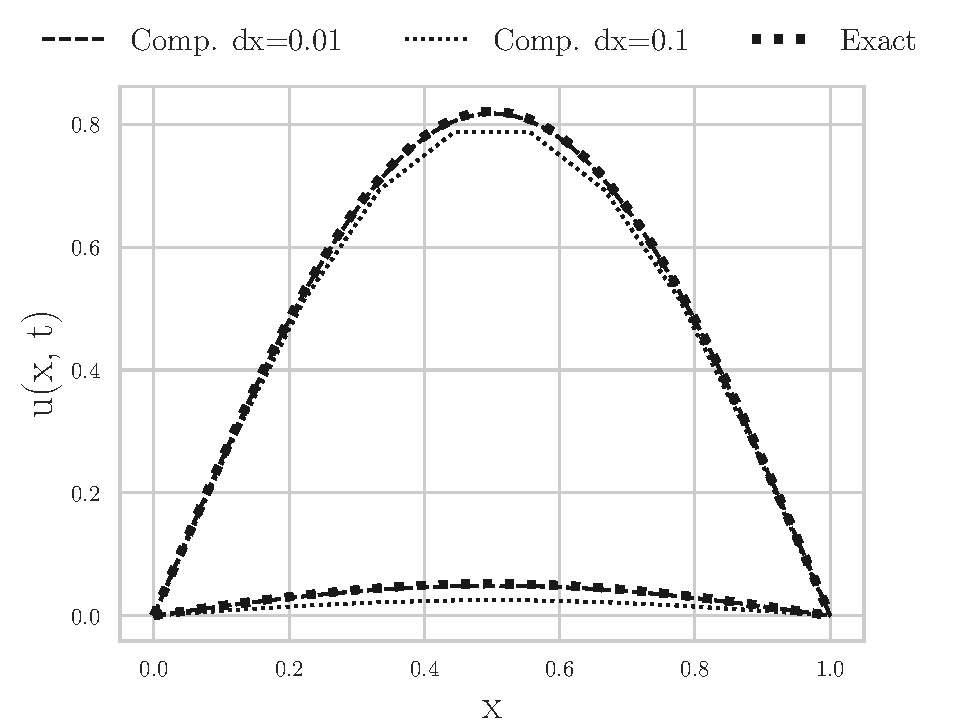
\includegraphics[width=0.5\textwidth]{FD_solved_new}
  	\caption{Time evolution of eq. \ref{eq:diffusionEQ} solved using finite difference methods: CD and FE for time's $t=0.02$ s and $t=0.3$ s. For each point in time a visual comparison is made with the exact solution.}
   \label{fig:FDcompare}
 \end{figure}

Likewise, in Figure \ref{fig:NNcompare} we show a parallell to Figure \ref{fig:FDcompare} with solutions from a neural network. In this case, we also see agreement between the computed and exact solutions for both points in time.
 \begin{figure}[htbp]
  	\centering
  	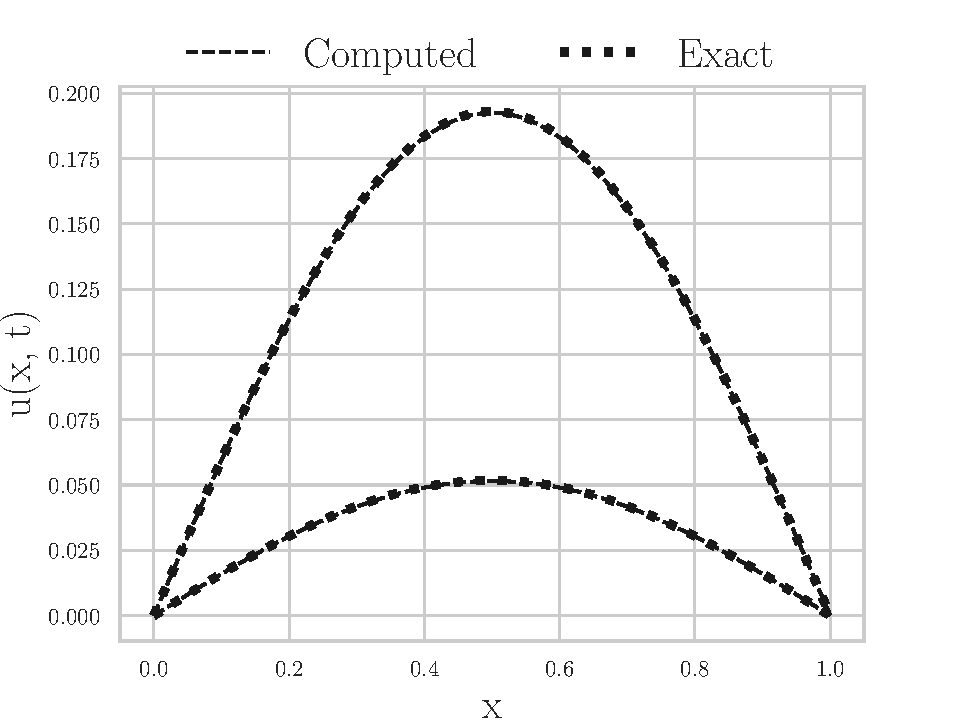
\includegraphics[width=0.5\textwidth]{NN_solved}
  	\caption{Time evolution of eq. \ref{eq:diffusionEQ} solved using a neural network. For both instants in time, $t=0.02$ s and $t=0.3$ s, a visual comparison is made with the exact solution, represented by dotted lines. The computations are done with $N_t = 30$ and $N_x = 100$.}
   \label{fig:NNcompare}
 \end{figure}

Shown in Figure \ref{fig:MSEbench} are the MSE's for two instants in time for both finite difference methods and a neural network. For the finite difference methods we observe a decrease in MSE for increasing temporal solution, slowing down after around 500 time points for both cases. For $t=0.02$ s (a.), the MSE is minimal at around $10^{-6}$ for 1000 time points, while for $t=0.3$ s (c.) it only becomes around $10^{-5}$ for 1000 time points.

For the neural network, we observe a decrease in MSE for an increasing number of iterations. In the case of $t=0.02$ s (b.), we see that the MSE decreases below $10^{-8}$ after around 6000 iterations, with a further, but slight, decrease at 10000 iterations. As for $t=0.3$ s (d.), the MSE is below $10^{-8}$ after around 4000 iterations and is mostly unchanged afterwards.

Comparison between the finite difference methods and the neural network, we see that the neural network can obtain an MSE 2-3 orders of magnitude lower than the finite difference methods.
\begin{figure}[htbp]
 	\centering
 	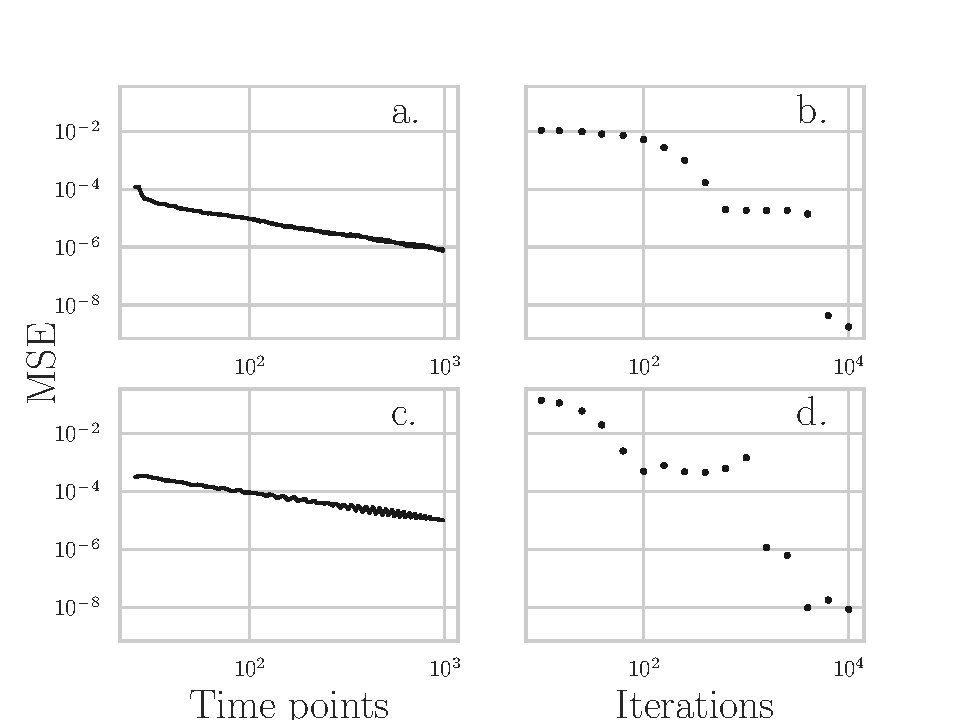
\includegraphics[width=0.5\textwidth]{MSEbench}
  \caption{Shown on the left-hand side, top-to-bottom (a., c.), are the MSE's as a function of temporal resolution, obtained from using finite difference methods for $t=0.02$ and $t=0.3$, respectively. Likewise, on the right-hand side (b., d.) the MSE's yielded from the neural network are shown as a function of iterations with network parameters $N_t = 10$, $N_x = 100$, and $\gamma = 0.004$.}
  \label{fig:MSEbench}
\end{figure}

Accompanying Figure \ref{fig:MSEbench}, we show the CPU times as a function of temporal resolution and number of iterations, respectively, for the different scenarios in Figure \ref{fig:CPUbench}. We see that the general curve is very similar for all scenarios. For the CD/FE method, we see that the CPU time becomes slightly longer for shorter t at 1000 time points. The neural network looks to have the same curve in both b. and d.

Comparing the two methods, we see that the neural network is around 3 orders of magnitude, if not more, slower than the finite difference methods.
\begin{figure}[htbp]
 	\centering
 	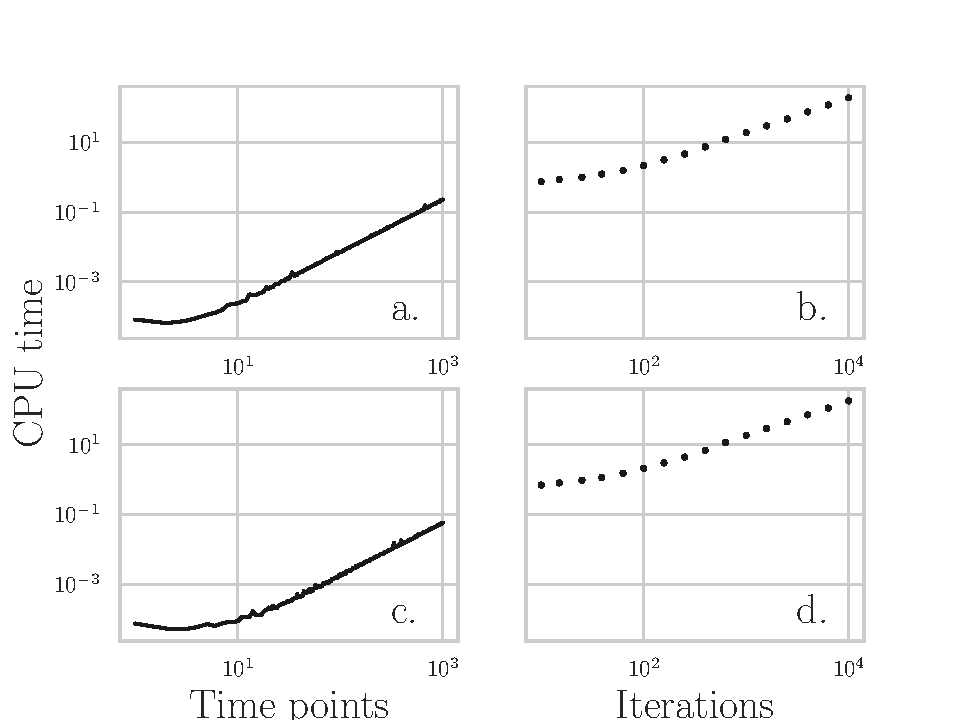
\includegraphics[width=0.5\textwidth]{CPUbench}
 	\caption{Shown on the left-hand side, top-to-bottom (a., c.), are the CPU time's as a function of temporal resolution, obtained from using finite difference methods for $t=0.02$ and $t=0.3$, respectively. Likewise, on the right-hand side (b., d.) the CPU time's yielded from the neural network are shown as a function of iterations with network parameters $N_t = 10$, $N_x = 100$, and $\gamma = 0.004$.}
  \label{fig:CPUbench}
\end{figure}


\subsection{Eigenpairs}
Looking at the eigenpairs of matrix A (\ref{matrix:A}), the maximum eigenvalue computed with  \texttt{numpy.linalg} is given under as $w_{max}^{np}$, with corresponding eigenvector $v_{max}^{np}$. The same eigenpair, computed with a neural network, is given as $w_{max}^{nn}$ and $v_{max}^{nn}$. Note that the eigenvectors have been normalized, to allow for comparison. We see that the two eigenvalues only differ at the 5th decimal place, while the eigenvector elements first differ at the 3th decimal place. Comparing the CPU times of the two methods for one run, the neural network is slower by a factor of about 1000.  

\begin{equation*}
v_{max}^{np} = \begin{bmatrix}
	0.4025950 \\
	0.4790814 \\
	0.3357358 \\
    0.3835011 \\
    0.3542414 \\
    0.4723555
\end{bmatrix} \quad w_{max}^{np} =  2.83515
\end{equation*}

\begin{equation*}
v_{max}^{nn} = \begin{bmatrix}
	0.40165637 \\
	0.47992723 \\
	0.33576365 \\
	0.38384145 \\
	0.35298366 \\
	0.47294087
\end{bmatrix} \quad w_{max}^{nn} = 2.83514
\end{equation*}

How $v_{max}^{nn}$ evolves over time is shown in Figure \ref{fig:eigenvector_max}. The network used for this computation had three hidden layers, all with ten neurons. The learning rate was 0.001, while the time step was 0.1. The precision, which was the MSE at which the training was stopped, was set to $10^{-4}$, resulting in 10820 iterations. 

 \begin{figure}[htbp]
 	\centering
 	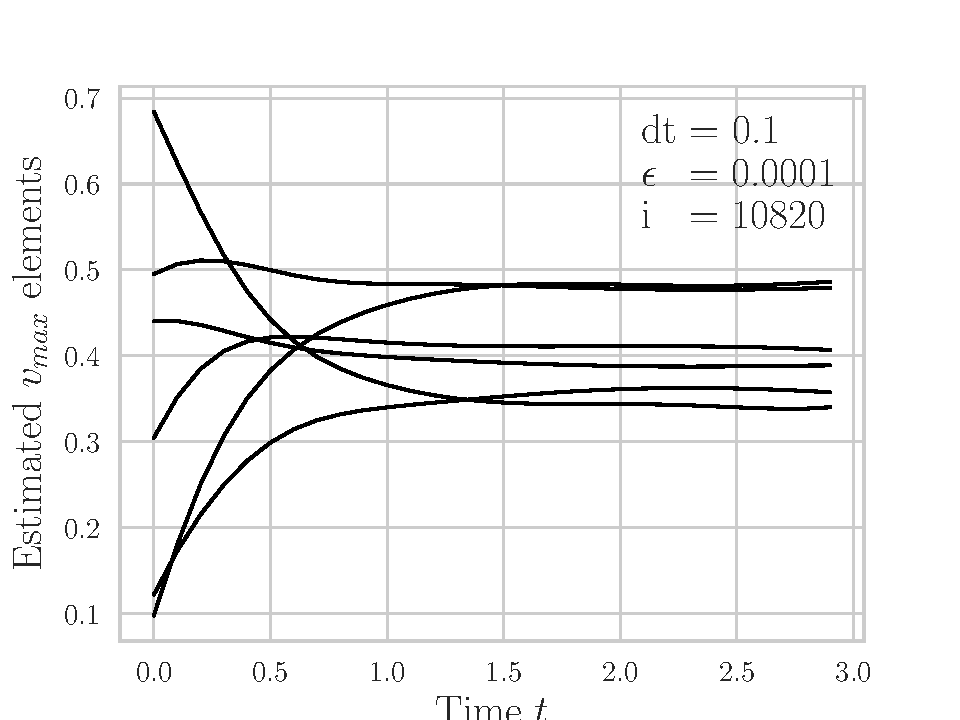
\includegraphics[width=0.5\textwidth]{eigenvector_max}
 	\caption{Figure showing how the value of the elements of the estimated eigenvector $v_{max}$ evolves over time, when computed by a neural network. Each line represents one of the elements of the vector. Time step $dt$, precision $\epsilon$ and iterations $i$ needed to achieve that precision is also shown.}
 	\label{fig:eigenvector_max}
 \end{figure}
 
 Analogously to what was shown above for the maximum eigenvalue, the minimum eigenvalue computed with \texttt{numpy.linalg} is shown below as $w_{min}^{np}$ together with the corresponding eigenvector $v_{min}^{np}$. Similarly, the same pair computed with neural network is denoted as $w_{min}^{nn}$ and $v_{min}^{nn}$. Again, the eigenvalues differ first at the 5th decimal place, and the egenvectors differ at the 3th decimal place, not taking the sign into account. 

\begin{equation*}
  v_{min}^{np} = \begin{bmatrix}
   0.6928048 \\
  -0.0074343 \\
  -0.7048516 \\
  -0.1487365 \\
  0.0122096 \\
  0.0296413
  \end{bmatrix} \quad w_{min}^{np} = -0.515594
\end{equation*}

\begin{equation*}
  v_{min}^{nn} = \begin{bmatrix}
   -0.69116113  \\
   0.00492352  \\
   0.70646873  \\
   0.14887754 \\
   -0.01982836 \\
   -0.02482513
  \end{bmatrix} \quad w_{min}^{nn} = -0.515528
\end{equation*}

Similarly to Figure \ref{fig:eigenvector_max}, the graph in Figure \ref{fig:eigenvector_min} shows the evolution of the eigenvector $v_{min}^{nn}$. Note the different time values in the two figures. The same network, with the same configurations as described above, is used, except that $A$ was replaced with $-A$ in the cost function. To reach a precision of $10^{-4}$, 842653 iterations was needed. 

\begin{figure}[htbp]
 \centering
 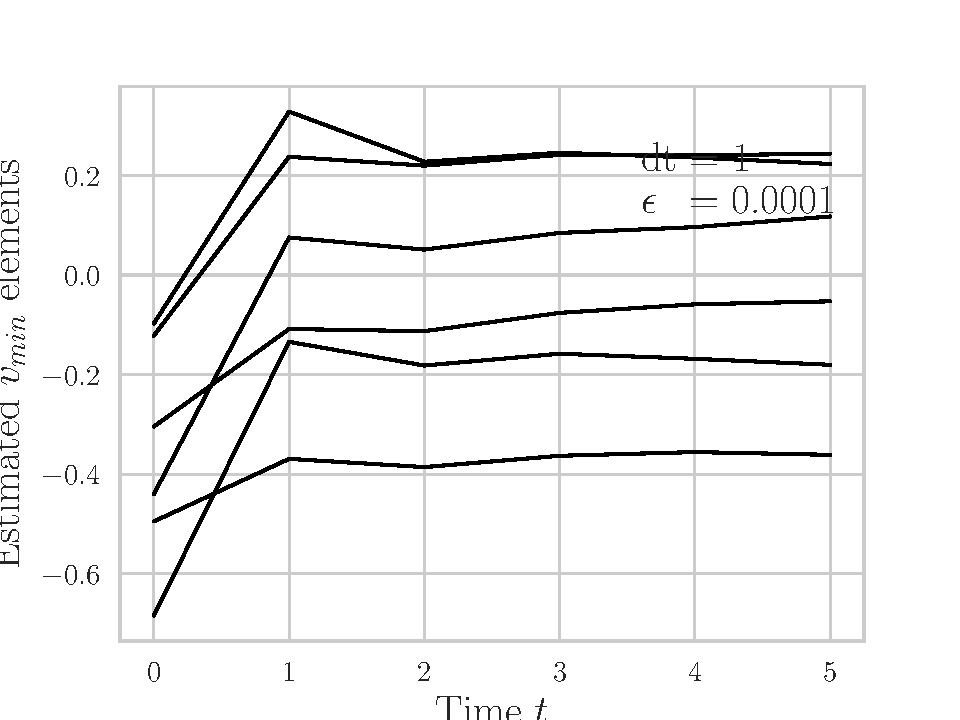
\includegraphics[width=0.5\textwidth]{eigenvector_min}
 \caption{Figure showing how the value of the elements of the estimated eigenvector $v_{min}$ evolves over time, when computed by a neural network. Each line represents one of the elements of the vector. Time step $dt$, precision $\epsilon$ and iterations $i$ needed to achieve that precision is also shown.}
 \label{fig:eigenvector_min}
\end{figure}

% Eksempel for figurer
% \begin{figure}[htbp]
% 	\centering
% 	\includegraphics[width=0.5\textwidth]{}
% 	\caption{}
% 	\label{fig:}
% \end{figure}
